Når data fra databasen skal læses, overskrives eller slettes bliver Repository-pattern og UnitOfWork benyttet - mere information omkring disse kan findes i \ref{Manglende reference}. I dette afsnit bliver det beskrevet, hvordan implementering af de forskellige CRUD-operationer på databasen er lavet. 
Da UnitOfWork og Repository-Pattern er blevet benyttet, betyder det, at al tilgang til databasen er stortset ens. Da databasen kun tilgås af UnitOfWork og GenericRepository.
Den ens tilgang til databasen betyder, at når data skal hentes i databasen skal der først oprettes et GenericRepository af den benyttede type (f.eks. UserRepository eller BarterAdRepository). 
Dette genericRepository benyttes som et håndtag til databasen, når der skal hentes data.

Over de følgende sider fremlægges sekvensdiagrammerne for, hvordan CRUD-operationerne er blevet udført for en barterad. Dette er et generelt eksempel og viser, hvordan database-trasaktionerne udføres.

\subsection{Create}
Et sekvensdiagram, for hvordan for eksempel en barterad oprettes og skrives i databasen ved brug af både UnitOfWork og GenericRepository, kan ses på figur \ref{fig:UOFSaveBarterAd}

\begin{figure}[H]
	\centering
	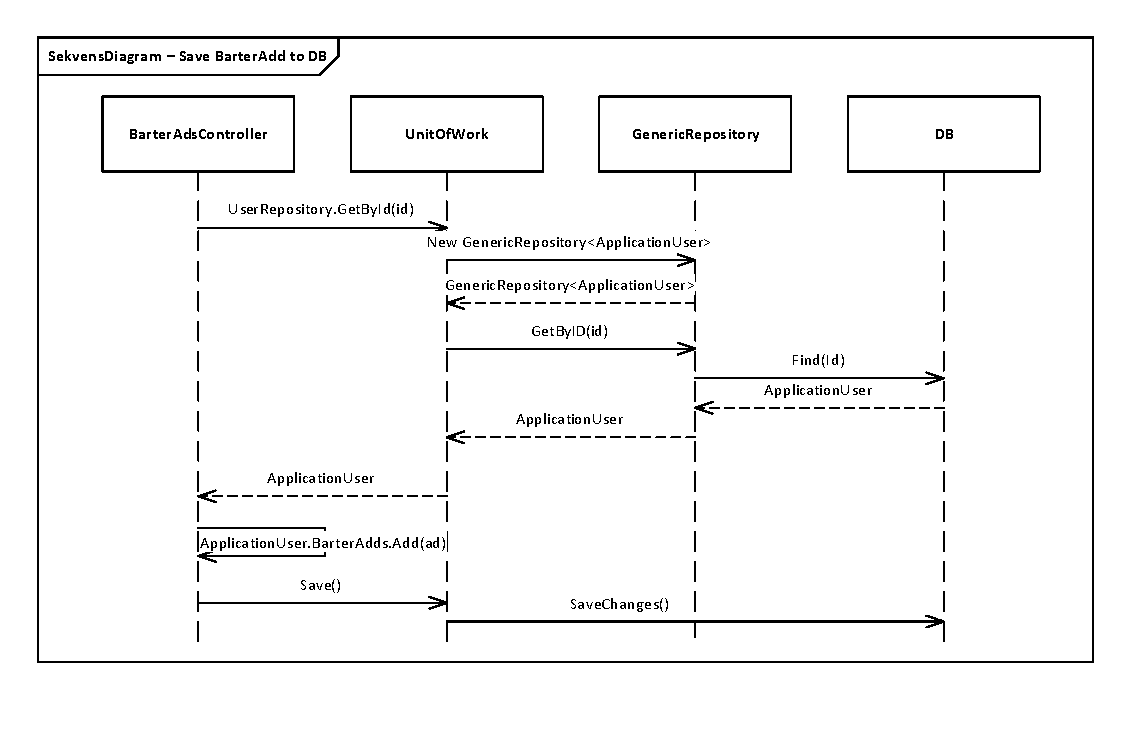
\includegraphics
	[width=150mm]{figures/SDUOFSaveBarterAd.PDF}
	\caption{Sekvensdiagram for, hvordan en barterAd bliver oprettet og gemt i DB}
	\label{fig:UOFSaveBarterAd}
\end{figure}
På sekvensdiagrammet figur \ref{fig:UOFSaveBarterAd} ses det, hvordan controlleren kalder over i unitofwork, der opretter et nyt genericrepository. Dette genericrepository gemmer barteraden i databasen.  


\subsection{Read} 
Et sekvensdiagram, for hvordan for eksempel en barterad findes og læses fra databasen ved brug af både UnitOfWork og GenericRepository, kan ses på figur \ref{fig:UOFFindBarterAd}

\begin{figure}[H]
	\centering
	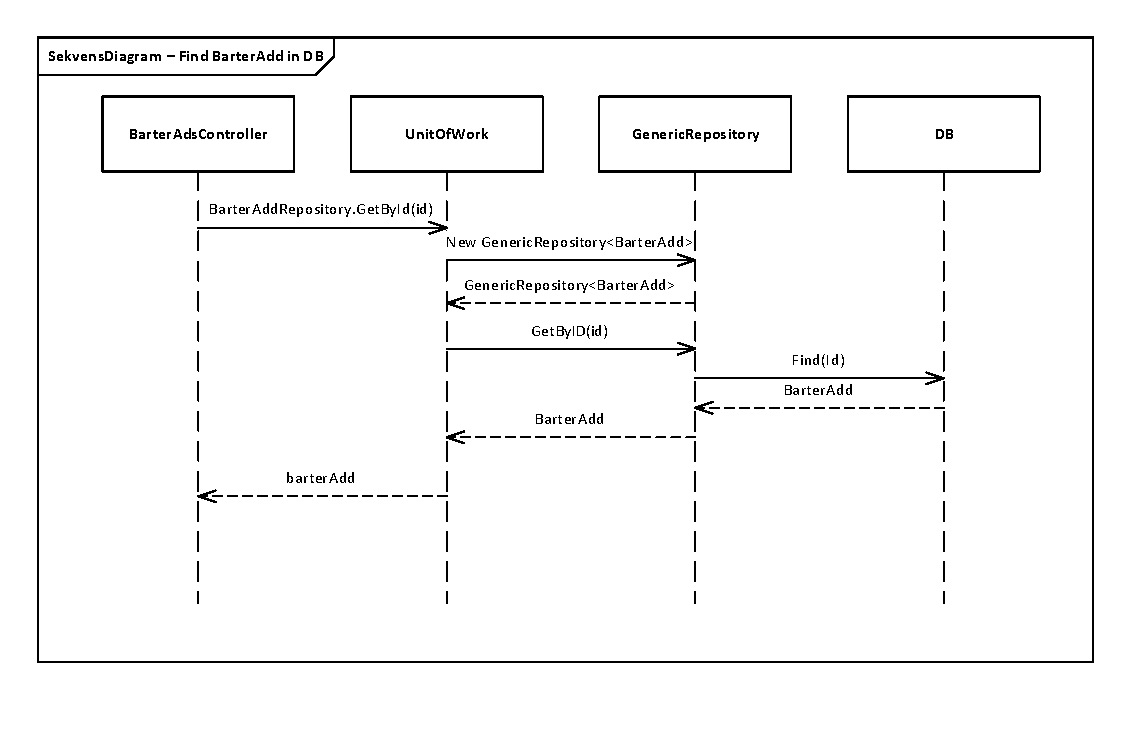
\includegraphics
	[width=150mm]{figures/SDUOFFindBarterAd.PDF}
	\caption{Sekvensdiagram for, hvordan en barterAd bliver fundet i DB}
	\label{fig:UOFFindBarterAd}
\end{figure}
På sekvensdiagrammet figur \ref{fig:UOFFindBarterAd} ses det, hvordan controlleren kalder over i unitofwork, der opretter et nyt genericrepository. Dette genericrepository finder barteraden i databasen.  


\subsection{Update}
Et sekvensdiagram, for hvordan for eksempel en barterad findes og opdateres i databasen ved brug af både UnitOfWork og GenericRepository, kan ses på figur \ref{fig:UOFUpdateBarterAd}
\begin{figure}[H]
	\centering
	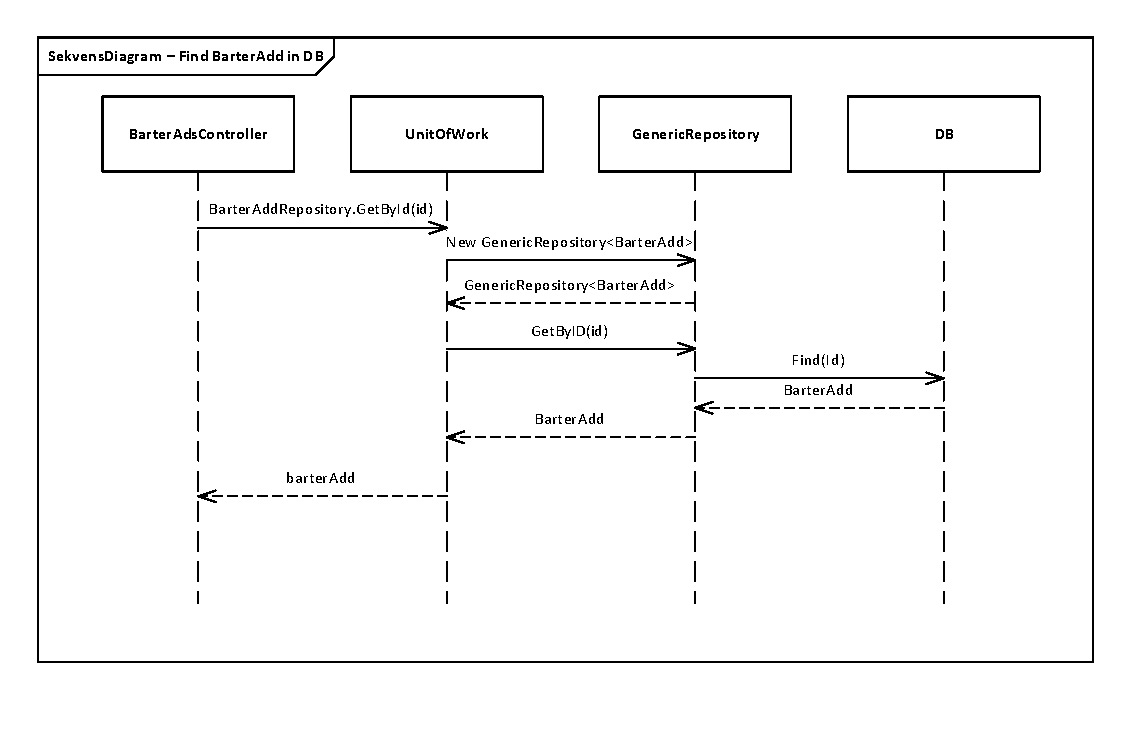
\includegraphics
	[width=150mm]{figures/SDUOFFindBarterAd.PDF}
	\caption{Sekvensdiagram for, hvordan en barterAd bliver opdateret i DB}
	\label{fig:UOFUpdateBarterAd}
\end{figure}
På sekvensdiagrammet figur \ref{fig:UOFUpdateBarterAd} ses det, hvordan controlleren kalder over i unitofwork, der opretter et nyt genericrepository. Dette genericrepository opdatere barteraden i databasen. 


\subsection{Delete}
Et sekvensdiagram, for hvordan for eksempel en barterad findes og slettes i databasen ved brug af både UnitOfWork og GenericRepository, kan ses på figur \ref{fig:UOFDeleteBarterAd}
\begin{figure}[H]
	\centering
	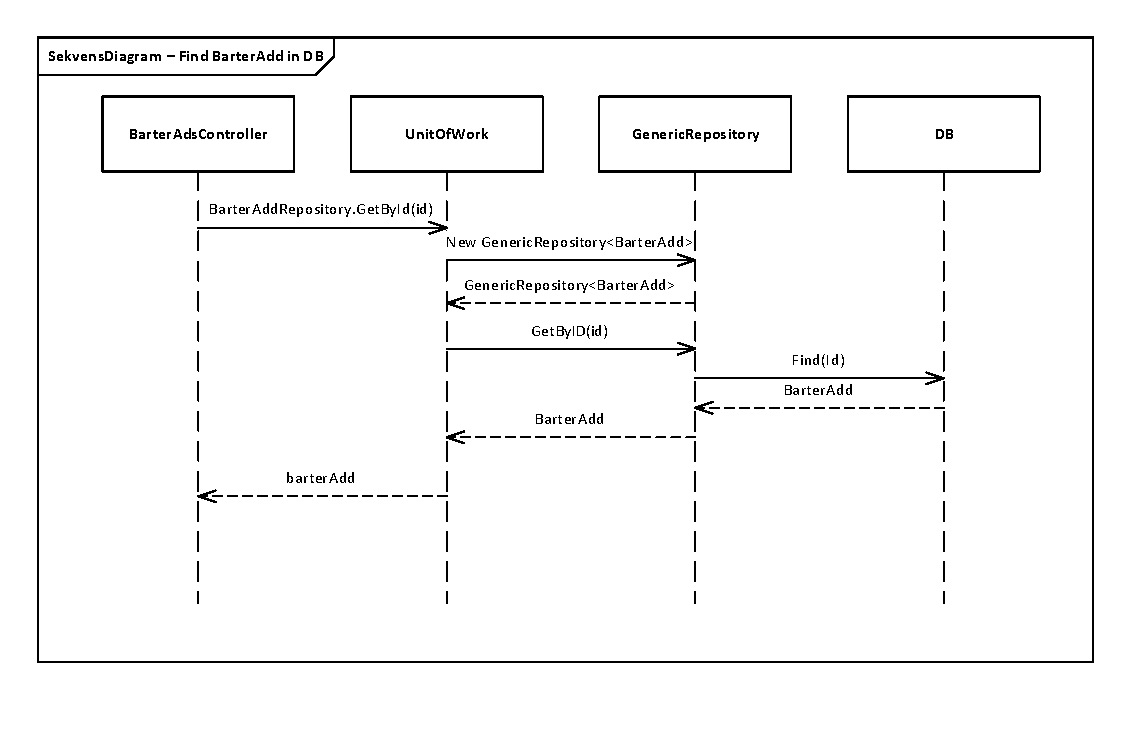
\includegraphics
	[width=145mm]{figures/SDUOFFindBarterAd.PDF}
	\caption{Sekvensdiagram for, hvordan en barterAd bliver slettet i DB}
	\label{fig:UOFDeleteBarterAd}
\end{figure}
På sekvensdiagrammet figur \ref{fig:UODeleteBarterAd} ses det, hvordan controlleren kalder over i unitofwork, der opretter et nyt genericrepository. Dette genericrepository sletter barteraden i databasen. 